\documentclass[aspectratio=169,14pt]{beamer}
\usetheme{default}
\usepackage{fontspec}
\setmainfont{texgyrepagella-regular.otf}[BoldFont=texgyrepagella-bold.otf,ItalicFont=texgyrepagella-italic.otf,BoldItalicFont=texgyrepagella-bolditalic.otf]
\setsansfont{texgyreheros-regular.otf}[BoldFont=texgyreheros-bold.otf,ItalicFont=texgyreheros-italic.otf,BoldItalicFont=texgyreheros-bold.otf,BoldItalicFeatures={FakeSlant=0.2}]
\setmonofont{lmmono10-regular.otf}[Scale=0.85]
\setbeamertemplate{navigation symbols}{}
\usepackage{pgfpages}
\newif\ifpresenter
\ifdefined\PresenterVersion\presentertrue\else\presenterfalse\fi
\ifpresenter
  \setbeameroption{show notes on second screen=right}
  \setbeamertemplate{note page}[plain]
\fi
\usepackage{amsmath,amssymb,bm,booktabs,array,graphicx,xcolor}
\usepackage{tikz,pgfplots,adjustbox,listings,xurl}
\pgfplotsset{compat=1.18}
\usetikzlibrary{arrows.meta,positioning,calc,fit,shapes.geometric,decorations.pathreplacing,patterns}
% UIUC official brand colors, verified 2026-10-23.
% https://brand.illinois.edu/visual-identity/color
\definecolor{IlliniOrange}{HTML}{FF5F05}
\definecolor{IlliniBlue}{HTML}{13294B}
\definecolor{Storm}{HTML}{707372}
\definecolor{LightStorm}{HTML}{C6C7C6}
\definecolor{Industrial}{HTML}{1D58A7}
\definecolor{Patina}{HTML}{007E8E}
\tikzset{>=Stealth, every node/.style={font=\small,text=IlliniBlue}, box/.style={draw=IlliniBlue,rounded corners=2pt,align=center,inner sep=6pt,execute at begin node=\hyphenpenalty10000\relax}, orangebox/.style={box,draw=IlliniOrange,very thick}, edge/.style={->,thick,IlliniBlue}, accent/.style={->,very thick,IlliniOrange}}
\pgfplotsset{every axis/.append style={width=13.5cm,height=6.5cm,axis line style={IlliniBlue},tick label style={font=\small,text=IlliniBlue},label style={font=\small,text=IlliniBlue},legend style={font=\small,draw=none,fill=white},grid style={LightStorm},major grid style={LightStorm},axis lines=left,clip=false}, every axis plot/.append style={thick}}

\definecolor{slidepaper}{RGB}{234,220,201}
\setbeamercolor{background canvas}{bg=slidepaper}
\setbeamercolor{normal text}{fg=IlliniBlue}
\setbeamercolor{frametitle}{fg=IlliniBlue}
\setbeamercolor{title}{fg=IlliniBlue}
\setbeamercolor{item}{fg=IlliniOrange}
\setbeamerfont{frametitle}{size=\large,series=\bfseries}
\setbeamerfont{title}{size=\Large,series=\bfseries}
\setbeamertemplate{itemize item}{\color{IlliniOrange}$\bullet$}
\setbeamertemplate{itemize subitem}{\color{IlliniOrange}\footnotesize$\circ$}
\setbeamercolor{orangerule}{bg=IlliniOrange}
\setbeamertemplate{headline}{\begin{beamercolorbox}[wd=\paperwidth,ht=0.1cm,dp=0.1cm]{orangerule}\end{beamercolorbox}}
\setbeamertemplate{footline}{\begin{beamercolorbox}[wd=\paperwidth,ht=0.1cm,dp=0.1cm]{orangerule}\end{beamercolorbox}}
\setbeamersize{text margin left=0.65cm,text margin right=0.65cm}
\setlength{\leftmargini}{1.1em}
\newenvironment{slidebullets}{\begin{itemize}\setlength\itemsep{0.8em}}{\end{itemize}}
\pgfplotsset{every axis/.append style={legend style={fill=slidepaper}}}
\lstdefinelanguage{CoursePython}{keywords={from,import,for,in,if,else,def,return,assert,True,False,None},sensitive=true,morecomment=[l]{\#},morestring=[b]',morestring=[b]"}
\lstset{language=CoursePython,basicstyle=\ttfamily\small,keywordstyle=\color{IlliniBlue}\bfseries,commentstyle=\color{Storm},stringstyle=\color{IlliniBlue},showstringspaces=false,breaklines=true,columns=fullflexible,keepspaces=true,frame=none,aboveskip=0.7em,belowskip=0.7em}
\newcommand{\E}{\mathbb E}
\newcommand{\Var}{\operatorname{Var}}
\newcommand{\Cov}{\operatorname{Cov}}
\hypersetup{colorlinks=true,urlcolor=IlliniBlue,linkcolor=IlliniBlue}

\title{Marketing Analytics}
\subtitle{Customer Data and Measurement}
\author{By Nathan Yang}
\date{Session 02}
\begin{document}
\begin{frame}
\titlepage
\end{frame}
\begin{frame}{A Customer-Activity Decision}
\usebeamercolor[fg]{normal text}
\vfill
\begin{slidebullets}
\item An mHealth manager wants to understand reduced recorded use.
\item The comparison follows the same eligible customers over time.
\item A missing record can reflect nonuse, incomplete observation, or data coverage.
\end{slidebullets}
\vfill
\note{Logging is an observable app behavior. Complete dietary consumption and health outcomes require additional measurement. A metric must state the population represented in each period.

M2, Section 2.1, Marketing Analytics Lecture Notes. \url{../06_Lecture_Notes/modules/M02_Customer_Data_and_Visualization.md}}
\end{frame}
\begin{frame}{A Customer Table}
\usebeamercolor[fg]{normal text}
\vfill
\begin{slidebullets}
\item Begin with the eligible-customer roster.
\item Aggregate events to the customer-period level.
\item Left join the summaries to the roster.
\item Fill zero only when absence has the defined meaning of no recorded event.
\end{slidebullets}
\vfill
\note{Starting from events omits customers with no observed events. Filling a missing nutrition measurement with zero changes its meaning. The roster and observation window establish the denominator.

M2, Section 2.2, Marketing Analytics Lecture Notes. \url{../06_Lecture_Notes/modules/M02_Customer_Data_and_Visualization.md}}
\end{frame}
\begin{frame}{Two Activity Measures}
\usebeamercolor[fg]{normal text}
\noindent Let $D_i$ be observed logging days and $T$ the calendar days in a common window.
\medskip
\[
L_i=\frac{D_i}{T},\qquad \bar L=\frac{1}{N}\sum_{i=1}^{N}L_i
\]
\medskip
\noindent Each eligible customer receives equal weight, including customers with no recorded days.
\note{The mean describes recorded use per available calendar day. Averaging only customers with positive D conditions on activity and can obscure declining use.

M2, Section 2.10, Marketing Analytics Lecture Notes. \url{../06_Lecture_Notes/modules/M02_Customer_Data_and_Visualization.md}}
\end{frame}
\begin{frame}{Conditional and Fixed Denominators}
\usebeamercolor[fg]{normal text}
\centering
\begingroup
\begin{adjustbox}{max width=0.98\textwidth,max totalheight=0.65\textheight}
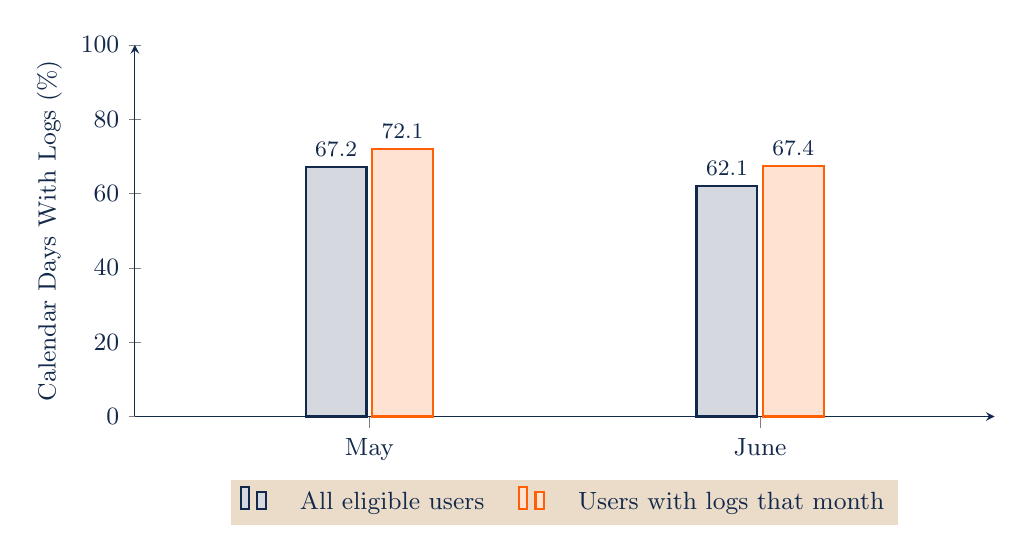
\begin{tikzpicture}
\begin{axis}[ybar,bar width=22pt,width=12.5cm,height=6.3cm,
 ymin=0,ymax=100,ylabel={Calendar Days With Logs (\%)},
 xtick={0,1},xticklabels={May,June},enlarge x limits=0.6,
 legend style={at={(0.5,-0.17)},anchor=north,legend columns=2,column sep=10pt},
 nodes near coords,point meta=y,
 every node near coord/.append style={font=\footnotesize,/pgf/number format/fixed,/pgf/number format/precision=1}]
\addplot[draw=IlliniBlue,fill=IlliniBlue!18] coordinates {(0.00000000,67.19165085) (1.00000000,62.06862745)};
\addplot[draw=IlliniOrange,fill=IlliniOrange!18] coordinates {(0.00000000,72.06675486) (1.00000000,67.42279020)};
\legend{All eligible users,Users with logs that month}
\end{axis}
\end{tikzpicture}

\end{adjustbox}
\endgroup
\par\medskip
{\small mHealth activity depends on who remains in the denominator.\par}
\note{The fixed cohort supports a comparison of changes in recorded use for the same customers. A conditional mean describes behavior among the customers still observed.

M2, Section 2.14, Marketing Analytics Lecture Notes. \url{../06_Lecture_Notes/modules/M02_Customer_Data_and_Visualization.md}}
\end{frame}
\begin{frame}{Repeated Totals}
\usebeamercolor[fg]{normal text}
\vfill
\begin{slidebullets}
\item An item row can contain a copied daily total.
\item Five copies of 1,132.79 sum to 5,663.95.
\item The item-calorie sum on that example day is 1,132.7852.
\end{slidebullets}
\vfill
\note{The five-fold inflation follows from repeated measurement fields, not a nutritional mechanism. One daily value can be retained after checking agreement within the user-day. Small rounding differences do not justify ignoring larger discrepancies.

M1, Section 1.8, Marketing Analytics Lecture Notes. \url{../06_Lecture_Notes/modules/M01_Marketing_Analytics_and_Python.md}}
\end{frame}
\begin{frame}{Structural Errors and Review Flags}
\usebeamercolor[fg]{normal text}
\vfill
\begin{slidebullets}
\item A duplicate daily key violates a one-row-per-day contract.
\item Equal item descriptions can represent repeated servings.
\item An extreme value warrants review under a stated rule.
\end{slidebullets}
\vfill
\note{Timestamp and meal identifiers are absent from the selected equality fields in the mHealth assessment. Dropping all equal records would impose a particular event definition. Preserve source values and add explicit flags.

M1, Section 1.8.3, Marketing Analytics Lecture Notes. \url{../06_Lecture_Notes/modules/M01_Marketing_Analytics_and_Python.md}}
\end{frame}
\begin{frame}[fragile]{A Fixed Customer Denominator}
\usebeamercolor[fg]{normal text}
\noindent Synthetic counts follow all four eligible customers.
\begin{lstlisting}
days = {'A': 20, 'B': 10, 'C': 0, 'D': 0}
fixed = sum(days.values()) / (4 * 30)
active = [x for x in days.values() if x > 0]
conditional = sum(active) / (len(active) * 30)
assert round(fixed, 4) == 0.25
assert round(conditional, 4) == 0.50
\end{lstlisting}
{\small The fixed-roster rate is 25\%. The active-user rate is 50\%.\par}
\note{Both numbers use the same observed days. The denominator changes from 120 potential customer-days to 60. These are synthetic counts.

M2, Section 2.1, Marketing Analytics Lecture Notes. \url{../06_Lecture_Notes/modules/M02_Customer_Data_and_Visualization.md}}
\end{frame}
\begin{frame}{Cohorts and Customer Age}
\usebeamercolor[fg]{normal text}
\vfill
\begin{slidebullets}
\item Group customers by a defined entry period.
\item Compare the same time since entry.
\item Mark later outcomes as unobserved when the horizon has not elapsed.
\end{slidebullets}
\vfill
\note{A recent cohort has no twelve-month outcome yet. Treating that cell as zero creates false attrition. The event defining entry must also remain stable across cohorts.

M2, Section 2.4, Marketing Analytics Lecture Notes. \url{../06_Lecture_Notes/modules/M02_Customer_Data_and_Visualization.md}}
\end{frame}
\begin{frame}{Retention Has a Triangular Support}
\usebeamercolor[fg]{normal text}
\centering
\begingroup
\fontsize{11}{13.2}\selectfont
\def\small{\fontsize{10}{12}\selectfont}
\def\footnotesize{\fontsize{9}{11}\selectfont}
\def\scriptsize{\fontsize{8}{9.5}\selectfont}
\hyphenpenalty=10000
\begin{adjustbox}{max width=0.98\textwidth,max totalheight=0.65\textheight}
% Original synthetic teaching figure; see corresponding module.
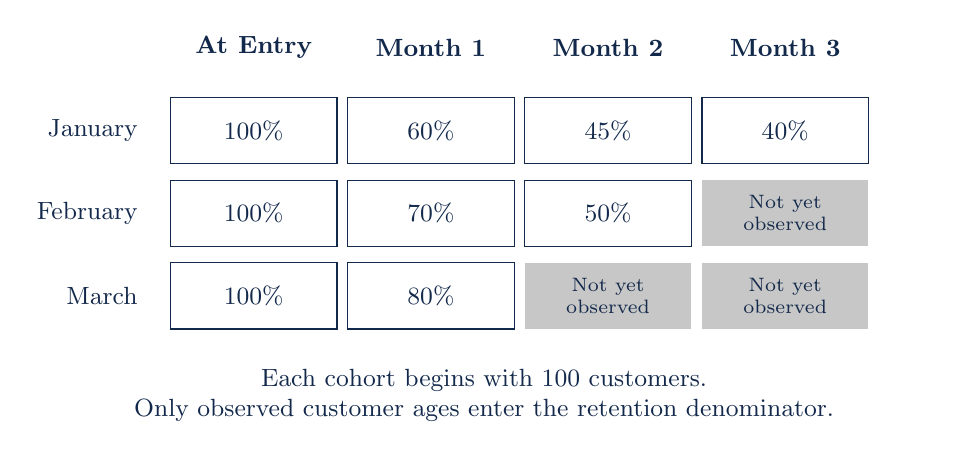
\begin{tikzpicture}[x=2.25cm,y=1.05cm]
\foreach \c/\lab in {0/At Entry,1/Month 1,2/Month 2,3/Month 3} {\node[font=\small\bfseries] at (\c,1) {\lab};}
\foreach \r/\lab in {0/January,-1/February,-2/March} {\node[anchor=east] at (-.6,\r) {\lab};}
\foreach \x/\y/\v in {0/0/100,1/0/60,2/0/45,3/0/40,0/-1/100,1/-1/70,2/-1/50,0/-2/100,1/-2/80} {\draw[IlliniBlue] (\x-.47,\y-.4) rectangle (\x+.47,\y+.4);\node at (\x,\y) {\v\%};}
\foreach \x/\y in {3/-1,2/-2,3/-2} {\fill[LightStorm] (\x-.47,\y-.4) rectangle (\x+.47,\y+.4);\node[align=center,font=\scriptsize] at (\x,\y) {Not yet\\observed};}
\node[align=center,text width=11cm] at (1.3,-3.2) {Each cohort begins with 100 customers.\\Only observed customer ages enter the retention denominator.};
\end{tikzpicture}

\end{adjustbox}
\endgroup
\par\medskip
{\small Synthetic cohort structure. Blank cells have no elapsed follow-up.\par}
\note{Calendar time, tenure, and acquisition cohort are different dimensions. A comparison at fixed tenure avoids giving newer customers shorter opportunities to remain active.

M2, Section 2.4, Marketing Analytics Lecture Notes. \url{../06_Lecture_Notes/modules/M02_Customer_Data_and_Visualization.md}}
\end{frame}
\begin{frame}{McBroken as a Measurement Case}
\usebeamercolor[fg]{normal text}
\vfill
\begin{slidebullets}
\item The records describe ice-cream ordering availability.
\item A missing snapshot has an unknown status.
\item Restaurant coverage and status recognition can change over time.
\end{slidebullets}
\vfill
\note{Order unavailability can reflect conditions besides a verified mechanical breakdown. A parser must distinguish known available, known unavailable, and unrecognized states. The source assessment and data dictionary define those categories.

M2, Section 2.16, Marketing Analytics Lecture Notes. \url{../06_Lecture_Notes/modules/M02_Customer_Data_and_Visualization.md}}
\end{frame}
\begin{frame}{Coverage Changes the Percentage}
\usebeamercolor[fg]{normal text}
\centering
\begingroup
\begin{adjustbox}{max width=0.98\textwidth,max totalheight=0.65\textheight}
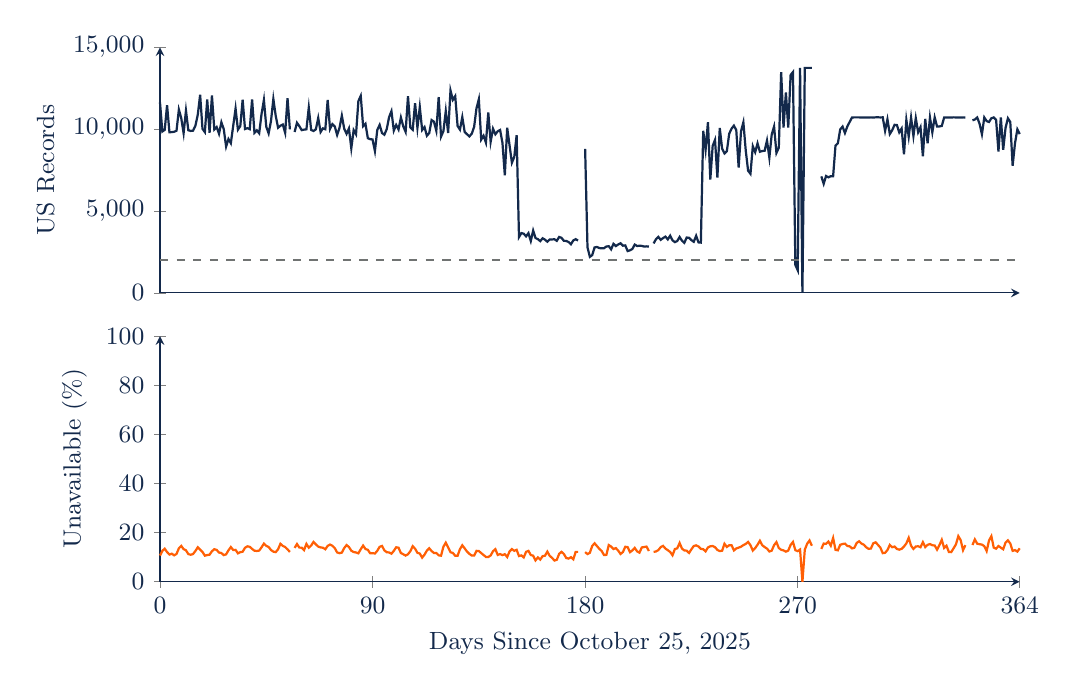
\begin{tikzpicture}
\begin{axis}[name=counts,width=12.5cm,height=4.7cm,xmin=0,xmax=364,
 ymin=0,ymax=15000,ylabel={US Records},xtick=\empty,scaled y ticks=false,
 ytick={0,5000,10000,15000},unbounded coords=jump]
\addplot[IlliniBlue] coordinates {(0,11640.000000) (1,9859.000000) (2,9959.000000) (3,11466.000000) (4,9814.000000) (5,9822.000000) (6,9842.000000) (7,9907.000000) (8,11199.000000) (9,10678.000000) (10,9757.000000) (11,11137.000000) (12,9937.000000) (13,9893.000000) (14,9909.000000) (15,10214.000000) (16,10883.000000) (17,12101.000000) (18,10021.000000) (19,9823.000000) (20,11810.000000) (21,9787.000000) (22,12057.000000) (23,9983.000000) (24,10132.000000) (25,9722.000000) (26,10421.000000) (27,10003.000000) (28,8940.000000) (29,9398.000000) (30,9147.000000) (31,10202.000000) (32,11260.000000) (33,9968.000000) (34,10184.000000) (35,11803.000000) (36,10011.000000) (37,10064.000000) (38,10000.000000) (39,11822.000000) (40,9779.000000) (41,9933.000000) (42,9750.000000) (43,10930.000000) (44,11794.000000) (45,10150.000000) (46,9745.000000) (47,10499.000000) (48,11847.000000) (49,10813.000000) (50,10089.000000) (51,10211.000000) (52,10287.000000) (53,9777.000000) (54,11895.000000) (55,9990.000000) (56,nan) (57,9828.000000) (58,10390.000000) (59,10187.000000) (60,9943.000000) (61,9972.000000) (62,9990.000000) (63,11318.000000) (64,9960.000000) (65,9889.000000) (66,9993.000000) (67,10686.000000) (68,9828.000000) (69,10049.000000) (70,9998.000000) (71,11786.000000) (72,10016.000000) (73,10308.000000) (74,10168.000000) (75,9649.000000) (76,10079.000000) (77,10827.000000) (78,10028.000000) (79,9717.000000) (80,10045.000000) (81,8831.000000) (82,9945.000000) (83,9690.000000) (84,11717.000000) (85,12035.000000) (86,10184.000000) (87,10330.000000) (88,9449.000000) (89,9391.000000) (90,9372.000000) (91,8659.000000) (92,9953.000000) (93,10263.000000) (94,9767.000000) (95,9661.000000) (96,10005.000000) (97,10736.000000) (98,11101.000000) (99,9914.000000) (100,10260.000000) (101,9982.000000) (102,10715.000000) (103,10172.000000) (104,9837.000000) (105,12017.000000) (106,10106.000000) (107,9963.000000) (108,11589.000000) (109,10084.000000) (110,11356.000000) (111,9951.000000) (112,10131.000000) (113,9600.000000) (114,9766.000000) (115,10557.000000) (116,10457.000000) (117,9899.000000) (118,11962.000000) (119,9547.000000) (120,9881.000000) (121,11108.000000) (122,9772.000000) (123,12366.000000) (124,11794.000000) (125,12023.000000) (126,10197.000000) (127,9974.000000) (128,10739.000000) (129,9830.000000) (130,9691.000000) (131,9560.000000) (132,9724.000000) (133,10139.000000) (134,11275.000000) (135,11832.000000) (136,9363.000000) (137,9600.000000) (138,9179.000000) (139,11020.000000) (140,9227.000000) (141,10029.000000) (142,9687.000000) (143,9874.000000) (144,9953.000000) (145,9162.000000) (146,7183.000000) (147,10091.000000) (148,9016.000000) (149,7953.000000) (150,8305.000000) (151,9634.000000) (152,3411.000000) (153,3653.000000) (154,3615.000000) (155,3454.000000) (156,3651.000000) (157,3170.000000) (158,3811.000000) (159,3351.000000) (160,3282.000000) (161,3161.000000) (162,3337.000000) (163,3252.000000) (164,3127.000000) (165,3262.000000) (166,3265.000000) (167,3277.000000) (168,3179.000000) (169,3416.000000) (170,3366.000000) (171,3181.000000) (172,3174.000000) (173,3107.000000) (174,2973.000000) (175,3206.000000) (176,3283.000000) (177,3196.000000) (178,nan) (179,nan) (180,8795.000000) (181,2780.000000) (182,2203.000000) (183,2306.000000) (184,2777.000000) (185,2805.000000) (186,2739.000000) (187,2722.000000) (188,2732.000000) (189,2832.000000) (190,2853.000000) (191,2659.000000) (192,2999.000000) (193,2861.000000) (194,2959.000000) (195,3033.000000) (196,2883.000000) (197,2901.000000) (198,2553.000000) (199,2600.000000) (200,2683.000000) (201,2951.000000) (202,2865.000000) (203,2880.000000) (204,2871.000000) (205,2828.000000) (206,2843.000000) (207,2826.000000) (208,nan) (209,3021.000000) (210,3281.000000) (211,3422.000000) (212,3242.000000) (213,3348.000000) (214,3438.000000) (215,3266.000000) (216,3494.000000) (217,3212.000000) (218,3100.000000) (219,3169.000000) (220,3415.000000) (221,3190.000000) (222,3059.000000) (223,3381.000000) (224,3364.000000) (225,3220.000000) (226,3122.000000) (227,3489.000000) (228,3085.000000) (229,3071.000000) (230,9900.000000) (231,8735.000000) (232,10426.000000) (233,6920.000000) (234,8982.000000) (235,9348.000000) (236,7041.000000) (237,10072.000000) (238,8810.000000) (239,8517.000000) (240,8654.000000) (241,9723.000000) (242,10036.000000) (243,10220.000000) (244,9932.000000) (245,7664.000000) (246,9872.000000) (247,10421.000000) (248,8702.000000) (249,7463.000000) (250,7273.000000) (251,8962.000000) (252,8599.000000) (253,9135.000000) (254,8622.000000) (255,8667.000000) (256,8682.000000) (257,9311.000000) (258,8260.000000) (259,9678.000000) (260,10165.000000) (261,8549.000000) (262,8869.000000) (263,13490.000000) (264,10097.000000) (265,12238.000000) (266,10097.000000) (267,13312.000000) (268,13491.000000) (269,1710.000000) (270,1388.000000) (271,13751.000000) (272,2.000000) (273,13746.000000) (274,13746.000000) (275,13746.000000) (276,13746.000000) (277,nan) (278,nan) (279,nan) (280,7120.000000) (281,6663.000000) (282,7141.000000) (283,7060.000000) (284,7128.000000) (285,7129.000000) (286,8999.000000) (287,9136.000000) (288,9988.000000) (289,10158.000000) (290,9767.000000) (291,10165.000000) (292,10443.000000) (293,10716.000000) (294,10722.000000) (295,10721.000000) (296,10721.000000) (297,10719.000000) (298,10719.000000) (299,10720.000000) (300,10714.000000) (301,10722.000000) (302,10716.000000) (303,10723.000000) (304,10725.000000) (305,10720.000000) (306,10724.000000) (307,9901.000000) (308,10603.000000) (309,9707.000000) (310,9935.000000) (311,10266.000000) (312,10252.000000) (313,9804.000000) (314,10041.000000) (315,8462.000000) (316,10562.000000) (317,9543.000000) (318,10711.000000) (319,9582.000000) (320,10677.000000) (321,9814.000000) (322,10125.000000) (323,8341.000000) (324,10632.000000) (325,9133.000000) (326,10713.000000) (327,9809.000000) (328,10721.000000) (329,10167.000000) (330,10170.000000) (331,10196.000000) (332,10711.000000) (333,10715.000000) (334,10710.000000) (335,10716.000000) (336,10723.000000) (337,10719.000000) (338,10719.000000) (339,10718.000000) (340,10721.000000) (341,10719.000000) (342,nan) (343,nan) (344,10545.000000) (345,10593.000000) (346,10716.000000) (347,10335.000000) (348,9693.000000) (349,10717.000000) (350,10493.000000) (351,10442.000000) (352,10670.000000) (353,10719.000000) (354,10567.000000) (355,8637.000000) (356,10721.000000) (357,8738.000000) (358,10082.000000) (359,10668.000000) (360,10442.000000) (361,7770.000000) (362,9143.000000) (363,9986.000000) (364,9702.000000)};
\addplot[Storm,dashed] coordinates {(0,2000) (364,2000)};
\end{axis}
\begin{axis}[at={(counts.south west)},anchor=north west,yshift=-0.55cm,
 width=12.5cm,height=4.7cm,xmin=0,xmax=364,ymin=0,ymax=100,
 ylabel={Unavailable (\%)},xlabel={Days Since October 25, 2025},
 xtick={0,90,180,270,364},unbounded coords=jump]
\addplot[IlliniOrange] coordinates {(0,10.661512) (1,12.577341) (2,13.445125) (3,12.087912) (4,11.065824) (5,11.423335) (6,10.760008) (7,11.315232) (8,13.635146) (9,14.609477) (10,13.272522) (11,12.795187) (12,11.271007) (13,10.987567) (14,11.292764) (15,12.531819) (16,14.021869) (17,13.073300) (18,12.134518) (19,10.617937) (20,10.863675) (21,11.024829) (22,12.424318) (23,13.252529) (24,12.949072) (25,11.880272) (26,11.697534) (27,10.826752) (28,11.174497) (29,12.789955) (30,14.135782) (31,12.948441) (32,12.984014) (33,11.567014) (34,12.048311) (35,12.225705) (36,13.824793) (37,14.417727) (38,14.230000) (39,13.381830) (40,12.649555) (41,12.533978) (42,12.697436) (43,14.016468) (44,15.516364) (45,14.591133) (46,14.171370) (47,12.925040) (48,12.256267) (49,12.059558) (50,13.222321) (51,15.463716) (52,14.591232) (53,14.145443) (54,13.198823) (55,12.142142) (56,nan) (57,13.776964) (58,15.351299) (59,13.909885) (60,13.869054) (61,12.886081) (62,15.415415) (63,13.880544) (64,14.738956) (65,16.220042) (66,15.200640) (67,14.327157) (68,13.970289) (69,13.852125) (70,13.222645) (71,14.610555) (72,15.145767) (73,14.639115) (74,13.699843) (75,11.928697) (76,11.638059) (77,11.868477) (78,13.711607) (79,14.942884) (80,14.146341) (81,12.637300) (82,12.106586) (83,11.919505) (84,11.572928) (85,13.236394) (86,14.728987) (87,13.349468) (88,12.985501) (89,11.585561) (90,11.651729) (91,11.490934) (92,12.609264) (93,14.225860) (94,14.579707) (95,12.783356) (96,12.023988) (97,11.922504) (98,11.422394) (99,12.557999) (100,14.035088) (101,13.874975) (102,11.684554) (103,11.197405) (104,10.663820) (105,11.200799) (106,12.438156) (107,14.463515) (108,13.461041) (109,11.781039) (110,11.465305) (111,9.828158) (112,11.035436) (113,12.677083) (114,13.628917) (115,12.494080) (116,11.714641) (117,11.698151) (118,10.750711) (119,10.610663) (120,14.269811) (121,15.916457) (122,13.958248) (123,12.016820) (124,11.734780) (125,10.563087) (126,10.571737) (127,13.274514) (128,14.843095) (129,13.591048) (130,12.269116) (131,11.349372) (132,10.674619) (133,10.642075) (134,12.585366) (135,12.508452) (136,11.673609) (137,10.895833) (138,10.099139) (139,10.072595) (140,10.707706) (141,12.423970) (142,13.265201) (143,10.917561) (144,11.262936) (145,10.849160) (146,11.220938) (147,10.068378) (148,12.344720) (149,13.290582) (150,12.594822) (151,13.006020) (152,10.466139) (153,10.730906) (154,9.903181) (155,12.188767) (156,12.571898) (157,10.883281) (158,10.627132) (159,8.713817) (160,9.902498) (161,9.016134) (162,10.428529) (163,10.608856) (164,12.280141) (165,10.545677) (166,9.739663) (167,8.635948) (168,8.933627) (169,11.358314) (170,12.180630) (171,11.317196) (172,9.672338) (173,9.430319) (174,9.989909) (175,9.139114) (176,12.153518) (177,12.171464) (178,nan) (179,nan) (180,12.075043) (181,11.258993) (182,11.802088) (183,14.570685) (184,15.664386) (185,14.545455) (186,13.399051) (187,12.527553) (188,10.871157) (189,10.946328) (190,14.931651) (191,14.328695) (192,13.337779) (193,13.701503) (194,12.673200) (195,11.308935) (196,12.105446) (197,14.236470) (198,14.101058) (199,12.038462) (200,12.746925) (201,13.791935) (202,12.390925) (203,11.840278) (204,13.967259) (205,14.144272) (206,14.315864) (207,12.526539) (208,nan) (209,12.148295) (210,12.343798) (211,12.887200) (212,14.096237) (213,14.605735) (214,13.525305) (215,12.859767) (216,12.135089) (217,10.772105) (218,13.322581) (219,13.600505) (220,15.783309) (221,13.510972) (222,12.749264) (223,12.658977) (224,11.712247) (225,13.229814) (226,14.541960) (227,14.817999) (228,14.359806) (229,13.415825) (230,13.232323) (231,12.375501) (232,13.974679) (233,14.436416) (234,14.562458) (235,14.077878) (236,12.938503) (237,12.480143) (238,12.644722) (239,15.463191) (240,14.166859) (241,14.861668) (242,14.876445) (243,12.759295) (244,13.552155) (245,13.896138) (246,14.262561) (247,14.921793) (248,15.398759) (249,16.213319) (250,14.876942) (251,12.698058) (252,13.699267) (253,15.062945) (254,16.689863) (255,14.860967) (256,14.132688) (257,13.500161) (258,12.324455) (259,12.657574) (260,14.913920) (261,16.142239) (262,13.733228) (263,13.017050) (264,12.776072) (265,12.240562) (266,12.716649) (267,14.993990) (268,16.210807) (269,12.865497) (270,12.463977) (271,13.119046) (272,0.000000) (273,13.021970) (274,15.480867) (275,16.804889) (276,14.658810) (277,nan) (278,nan) (279,nan) (280,13.356742) (281,15.548552) (282,15.432012) (283,16.359773) (284,14.688552) (285,17.814560) (286,13.001445) (287,12.806480) (288,15.058070) (289,15.367198) (290,15.521655) (291,14.589277) (292,14.421143) (293,13.587159) (294,13.850028) (295,15.810092) (296,16.490999) (297,15.542495) (298,15.094692) (299,14.029851) (300,13.393690) (301,13.542250) (302,15.668160) (303,16.058939) (304,14.993007) (305,13.908582) (306,11.646774) (307,11.786688) (308,12.902009) (309,15.009787) (310,14.051334) (311,14.328853) (312,13.353492) (313,13.066095) (314,13.405039) (315,14.370125) (316,15.603105) (317,17.908415) (318,14.657828) (319,13.368817) (320,14.348600) (321,14.448747) (322,14.054321) (323,16.125165) (324,14.136569) (325,15.022446) (326,15.364510) (327,14.863900) (328,14.756086) (329,13.071703) (330,14.916421) (331,17.075324) (332,13.742881) (333,14.652357) (334,12.128852) (335,12.066069) (336,13.624918) (337,15.215972) (338,18.565165) (339,16.962120) (340,12.853279) (341,14.898778) (342,nan) (343,nan) (344,14.964438) (345,17.247239) (346,15.490855) (347,15.287857) (348,15.124317) (349,14.481665) (350,12.494044) (351,16.816702) (352,18.556701) (353,13.900550) (354,13.466452) (355,14.542086) (356,13.888630) (357,13.241016) (358,15.949216) (359,16.854143) (360,15.590883) (361,12.574003) (362,12.884174) (363,12.277188) (364,13.605442)};
\end{axis}
\end{tikzpicture}

\end{adjustbox}
\endgroup
\par\medskip
{\small McBroken comparisons preserve the observed-store denominator.\par}
\note{A change in the set of included restaurants can change the national share without a within-restaurant change. Common-support comparisons answer a narrower population question.

M2, Section 2.16.1, Marketing Analytics Lecture Notes. \url{../06_Lecture_Notes/modules/M02_Customer_Data_and_Visualization.md}}
\end{frame}
\begin{frame}{Identity Across Files}
\usebeamercolor[fg]{normal text}
\vfill
\begin{slidebullets}
\item A restaurant address is a candidate key that requires checks.
\item Standardizing spelling can repair formatting differences.
\item Overaggressive matching can merge separate locations.
\end{slidebullets}
\vfill
\note{Track duplicates before and after normalization. Location identity and status measurement are separate tasks. A unique normalized string does not alone prove a unique physical establishment.

M2, Section 2.16.2, Marketing Analytics Lecture Notes. \url{../06_Lecture_Notes/modules/M02_Customer_Data_and_Visualization.md}}
\end{frame}
\begin{frame}{Coding Exercise: A Data Assessment}
\usebeamercolor[fg]{normal text}
\vfill
\begin{slidebullets}
\item Construct a roster-first activity table.
\item Report key uniqueness, unmatched rows, and zero-event customers.
\item Compare the fixed and conditional activity measures.
\end{slidebullets}
\vfill
\note{Run ../03\_Data\_and\_Code/Lecture\_Examples/session\_examples.py S02 for the hand-checkable example. For the real case, use the mHealth common.py and m01.py programs in the stated dependency order. Their full source and environment appear in the lecture notes.

M2, Section 2.10, Marketing Analytics Lecture Notes. \url{../06_Lecture_Notes/modules/M02_Customer_Data_and_Visualization.md}}
\end{frame}
\begin{frame}{AI Review of a Parser}
\usebeamercolor[fg]{normal text}
\vfill
\begin{slidebullets}
\item Supply the allowed statuses and a tiny labeled example.
\item Require an explicit unknown category for new statuses.
\item Compare parsed totals with an independently calculated source total.
\end{slidebullets}
\vfill
\note{A program that treats every unrecognized status as available can create artificial improvements. A counterexample containing a new status tests this failure directly.

M2, Section 2.16.3, Marketing Analytics Lecture Notes. \url{../06_Lecture_Notes/modules/M02_Customer_Data_and_Visualization.md}}
\end{frame}
\begin{frame}{A Data Dictionary for Decisions}
\usebeamercolor[fg]{normal text}
\vfill
\begin{slidebullets}
\item State the unit, key, timing, and units of each variable.
\item Record source versions and transformation rules.
\item Separate observed values, calculated quantities, and imposed assumptions.
\end{slidebullets}
\vfill
\note{A reader should be able to trace a plotted rate to its numerator and denominator without guessing the meaning of a field name.

M2, Section 2.2, Marketing Analytics Lecture Notes. \url{../06_Lecture_Notes/modules/M02_Customer_Data_and_Visualization.md}}
\end{frame}
\begin{frame}{Privacy and Collection Choices}
\usebeamercolor[fg]{normal text}
\vfill
\begin{slidebullets}
\item Collect the fields needed for the stated decision.
\item Retain source permissions and deletion or retention conditions.
\item Check whether a linkage increases the risk of identifying a person.
\end{slidebullets}
\vfill
\note{Combining datasets can change what can be inferred even when each file omits names. Data minimization is part of the analytical design, and dataset-specific restrictions remain applicable.

ETHICS\_AND\_REGULATION.md, M2.}
\end{frame}
\begin{frame}{Measurement Discussion}
\usebeamercolor[fg]{normal text}
\vfill
\begin{slidebullets}
\item Could recorded activity rise because low-activity users disappear?
\item Would deleting unmatched days change the target population?
\item What evidence would establish a mechanical failure?
\end{slidebullets}
\vfill
\note{Conditioning on observed users can raise activity among those remaining. An inner join changes the observed food-log population. A verified failure diagnosis requires information beyond online ordering availability.

M2, Section 2.16, Marketing Analytics Lecture Notes. \url{../06_Lecture_Notes/modules/M02_Customer_Data_and_Visualization.md}}
\end{frame}
\end{document}
